

\tikzset{every picture/.style={line width=0.75pt}} %set default line width to 0.75pt        

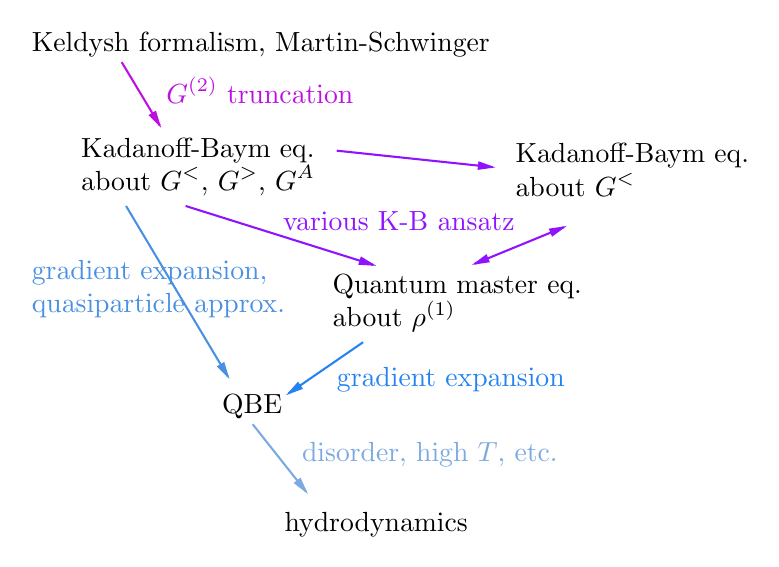
\begin{tikzpicture}[x=0.75pt,y=0.75pt,yscale=-0.7,xscale=0.7]
%uncomment if require: \path (0,409); %set diagram left start at 0, and has height of 409

%Straight Lines [id:da9993448313111608] 
\draw [color={rgb, 255:red, 189; green, 16; blue, 224 }  ,draw opacity=1 ]   (100,52) -- (126.14,95.47) ;
\draw [shift={(127.17,97.19)}, rotate = 238.99] [fill={rgb, 255:red, 189; green, 16; blue, 224 }  ,fill opacity=1 ][line width=0.08]  [draw opacity=0] (12,-3) -- (0,0) -- (12,3) -- cycle    ;
%Straight Lines [id:da505450204640074] 
\draw [color={rgb, 255:red, 144; green, 19; blue, 254 }  ,draw opacity=1 ]   (144,151) -- (273.26,191.59) ;
\draw [shift={(275.17,192.19)}, rotate = 197.43] [fill={rgb, 255:red, 144; green, 19; blue, 254 }  ,fill opacity=1 ][line width=0.08]  [draw opacity=0] (12,-3) -- (0,0) -- (12,3) -- cycle    ;
%Straight Lines [id:da7259646168352232] 
\draw [color={rgb, 255:red, 74; green, 144; blue, 226 }  ,draw opacity=1 ]   (103,151) -- (173.14,268.47) ;
\draw [shift={(174.17,270.19)}, rotate = 239.16] [fill={rgb, 255:red, 74; green, 144; blue, 226 }  ,fill opacity=1 ][line width=0.08]  [draw opacity=0] (12,-3) -- (0,0) -- (12,3) -- cycle    ;
%Straight Lines [id:da35768014069365206] 
\draw [color={rgb, 255:red, 36; green, 131; blue, 241 }  ,draw opacity=1 ]   (266.17,244.78) -- (214.82,280.06) ;
\draw [shift={(213.17,281.19)}, rotate = 325.51] [fill={rgb, 255:red, 36; green, 131; blue, 241 }  ,fill opacity=1 ][line width=0.08]  [draw opacity=0] (12,-3) -- (0,0) -- (12,3) -- cycle    ;
%Straight Lines [id:da15985835431985884] 
\draw [color={rgb, 255:red, 124; green, 170; blue, 224 }  ,draw opacity=1 ]   (190.17,301.25) -- (226.93,347.68) ;
\draw [shift={(228.17,349.25)}, rotate = 231.63] [fill={rgb, 255:red, 124; green, 170; blue, 224 }  ,fill opacity=1 ][line width=0.08]  [draw opacity=0] (12,-3) -- (0,0) -- (12,3) -- cycle    ;
%Straight Lines [id:da33183770683384806] 
\draw [color={rgb, 255:red, 144; green, 19; blue, 254 }  ,draw opacity=1 ]   (248,112.94) -- (355.18,124.25) ;
\draw [shift={(357.17,124.46)}, rotate = 186.02] [fill={rgb, 255:red, 144; green, 19; blue, 254 }  ,fill opacity=1 ][line width=0.08]  [draw opacity=0] (12,-3) -- (0,0) -- (12,3) -- cycle    ;
%Straight Lines [id:da43680180859475204] 
\draw [color={rgb, 255:red, 144; green, 19; blue, 254 }  ,draw opacity=1 ]   (404.32,165.61) -- (343.02,190.76) ;
\draw [shift={(341.17,191.52)}, rotate = 337.69] [fill={rgb, 255:red, 144; green, 19; blue, 254 }  ,fill opacity=1 ][line width=0.08]  [draw opacity=0] (12,-3) -- (0,0) -- (12,3) -- cycle    ;
\draw [shift={(406.17,164.85)}, rotate = 157.69] [fill={rgb, 255:red, 144; green, 19; blue, 254 }  ,fill opacity=1 ][line width=0.08]  [draw opacity=0] (12,-3) -- (0,0) -- (12,3) -- cycle    ;

% Text Node
\draw (36,29) node [anchor=north west][inner sep=0.75pt]   [align=left] {Keldysh formalism, Martin-Schwinger};
% Text Node
\draw (195.1,71.44) node  [color={rgb, 255:red, 189; green, 16; blue, 224 }  ,opacity=1 ] [align=left] {$\displaystyle G^{( 2)}$ truncation};
% Text Node
\draw (70,102) node [anchor=north west][inner sep=0.75pt]   [align=left] {Kadanoff-Baym eq.\\about $\displaystyle G^{< }$, $\displaystyle G^{ >}$, $\displaystyle G^{\text{A}}$};
% Text Node
\draw (209,153) node [anchor=north west][inner sep=0.75pt]  [color={rgb, 255:red, 144; green, 19; blue, 254 }  ,opacity=1 ] [align=left] {various K-B ansatz};
% Text Node
\draw (243,196) node [anchor=north west][inner sep=0.75pt]   [align=left] {Quantum master eq.\\about $\displaystyle \rho ^{( 1)}$};
% Text Node
\draw (36,186) node [anchor=north west][inner sep=0.75pt]  [color={rgb, 255:red, 74; green, 144; blue, 226 }  ,opacity=1 ] [align=left] {gradient expansion,\\quasiparticle approx.};
% Text Node
\draw (167,279) node [anchor=north west][inner sep=0.75pt]   [align=left] {QBE};
% Text Node
\draw (246,260) node [anchor=north west][inner sep=0.75pt]  [color={rgb, 255:red, 36; green, 131; blue, 241 }  ,opacity=1 ] [align=left] {gradient expansion};
% Text Node
\draw (222,311.45) node [anchor=north west][inner sep=0.75pt]  [color={rgb, 255:red, 124; green, 170; blue, 224 }  ,opacity=1 ] [align=left] {disorder, high $\displaystyle T$, etc.};
% Text Node
\draw (210,359.45) node [anchor=north west][inner sep=0.75pt]   [align=left] {hydrodynamics};
% Text Node
\draw (369,106) node [anchor=north west][inner sep=0.75pt]   [align=left] {Kadanoff-Baym eq.\\about $\displaystyle G^{< }$};


\end{tikzpicture}
